% ============================================================
%  EXECUTIVE PRESENTATION — PhD Defence
%  AI-Driven Intelligent Routing and Secure Autonomous Recovery
%  in 6G-Integrated Disaster-Monitoring Sensor Networks
%  Polytechnique Montréal — LARIM   |   Friday May 15 2026
%  Audience: Non-technical executives, Telecommunications Mobility
% ============================================================
\documentclass[aspectratio=169,t,10pt]{beamer}

% ---- Theme --------------------------------------------------
\usetheme{Madrid}
\usecolortheme{whale}

% ---- Packages -----------------------------------------------
\usepackage[utf8]{inputenc}
\usepackage[T1]{fontenc}
\usepackage{lmodern}
\usepackage{booktabs}
\usepackage{array}
\usepackage{xcolor}
\usepackage{graphicx}
\usepackage{tikz}
\usetikzlibrary{arrows.meta,positioning,shapes.geometric}
\usepackage{fontawesome5}
\usepackage{amsmath}
\usepackage{microtype}
\usepackage{colortbl}

% ---- Polytechnique colours ----------------------------------
\definecolor{polyblue}{RGB}{0,62,115}
\definecolor{polyred}{RGB}{206,17,38}
\definecolor{polygreen}{RGB}{0,105,55}
\definecolor{polyyellow}{RGB}{255,195,0}
\definecolor{lightbg}{RGB}{240,245,252}
\definecolor{alertred}{RGB}{180,0,0}
\definecolor{darkgreen}{RGB}{0,100,0}
\definecolor{lightgreen}{RGB}{228,244,228}
\definecolor{lightred}{RGB}{245,228,228}

% ---- Apply Polytechnique palette ----------------------------
\setbeamercolor{palette primary}{bg=polyblue,fg=white}
\setbeamercolor{palette secondary}{bg=polyblue!80,fg=white}
\setbeamercolor{palette tertiary}{bg=polyblue!60,fg=white}
\setbeamercolor{palette quaternary}{bg=polyblue,fg=white}
\setbeamercolor{structure}{fg=polyblue}
\setbeamercolor{section in toc}{fg=polyblue}
\setbeamercolor{frametitle}{bg=polyblue,fg=white}
\setbeamercolor{title}{bg=polyblue,fg=white}
\setbeamercolor{block title}{bg=polyblue,fg=white}
\setbeamercolor{block body}{bg=lightbg,fg=black}
\setbeamercolor{block title alerted}{bg=alertred,fg=white}
\setbeamercolor{block body alerted}{bg=lightred,fg=black}
\setbeamercolor{block title example}{bg=darkgreen,fg=white}
\setbeamercolor{block body example}{bg=lightgreen,fg=black}

% ---- Logo in footer -----------------------------------------
\addtobeamertemplate{footline}{}{%
  \hspace*{\fill}%
  \raisebox{3pt}{%
    
\includegraphics[height=0.38cm]{Polytechnique_Montreal_Logo.png}\hspace{4pt}%
    
\includegraphics[height=0.38cm]{Larim_logo.png}%
  }\hspace{6pt}%
}

% ---- Navigation symbols off ---------------------------------
\setbeamertemplate{navigation symbols}{}

% ---- Tighter margins to prevent content cuts ----------------
\setbeamersize{text margin left=0.55cm, text margin right=0.55cm}

% ============================================================
%  METADATA
% ============================================================
\title[AI-Driven 6G Disaster Networks]{%
  AI-Driven Intelligent Routing and Secure\\
  Autonomous Recovery in 6G-Integrated\\
  Disaster-Monitoring Sensor Networks%
}
\subtitle{PhD Defence}
\author[G.\,P. Djimefo Kapen]{%
  \textbf{Georges Parfait Djimefo Kapen}\\[3pt]
  {\small Director: \textbf{Ranwa Al-Mallah} \quad
         Co-director: \textbf{Samuel Pierre} \quad
         Supervisor: \textbf{Franjieh El-Khoury}}%
}
\institute[Polytechnique Montr\'eal]{%
  Department of Computer and Software Engineering \quad
  Polytechnique Montr\'eal~--~LARIM%
}
\date{Friday, May 15, 2026}

% ============================================================
\begin{document}
% ============================================================

% ---- Title slide --------------------------------------------
{
\setbeamertemplate{footline}{}
\begin{frame}[plain]
  \titlepage
  \begin{tikzpicture}[remember picture, overlay]
    \node[anchor=south east, inner sep=10pt]
      at (current page.south east) {%
        
\includegraphics[height=0.75cm]{Polytechnique_Montreal_Logo.png}%
        \hspace{6pt}%
        
\includegraphics[height=0.75cm]{Larim_logo.png}%
      };
  \end{tikzpicture}
\end{frame}
}

% ---- Agenda -------------------------------------------------
\begin{frame}{Agenda}
  \tableofcontents[hideallsubsections]
\end{frame}

% ============================================================
\section{Problem and Research Question}
% ============================================================

\begin{frame}[shrink=5]{The Problem: Networks Fail When Lives Are at Stake}
\begin{block}{\faExclamationTriangle\; The Disaster Coverage Gap}
  \begin{columns}[T]
  \begin{column}{0.48\textwidth}
    \begin{itemize}\small\setlength{\itemsep}{5pt}
      \item Natural disasters cause \textbf{\$300B\,+/year} in global losses
      \item Sensor networks deployed for monitoring
            \textbf{drain their batteries within hours} under disaster load
    \end{itemize}
  \end{column}
  \begin{column}{0.48\textwidth}
    \begin{itemize}\small\setlength{\itemsep}{5pt}
      \item Connectivity collapses exactly when \textbf{emergency calls}
            and alerts are most critical
      \item Sending field crews into a disaster zone
            is \textbf{dangerous and very costly}
    \end{itemize}
  \end{column}
  \end{columns}
\end{block}
\vspace{6pt}
\begin{alertblock}{\faBriefcase\; Why This Is a Mobility Operator Problem}
  \begin{columns}[T]
  \begin{column}{0.48\textwidth}
    \begin{itemize}\small\setlength{\itemsep}{4pt}
      \item \textbf{Coverage liability:} emergency call failures during crises
      \item \textbf{OPEX pressure:} frequent battery swaps and field maintenance
    \end{itemize}
  \end{column}
  \begin{column}{0.48\textwidth}
    \begin{itemize}\small\setlength{\itemsep}{4pt}
      \item \textbf{ESG gap:} no standardized carbon metric for sensor networks
      \item \textbf{Compliance risk:} AI-managed networks lack certified guardrails
    \end{itemize}
  \end{column}
  \end{columns}
\end{alertblock}
\vspace{6pt}
\begin{exampleblock}{The Core Gap}
  \centering\small
  Existing solutions \textbf{cannot simultaneously} guarantee high data delivery,
  minimize carbon cost, and protect AI-managed networks from compromise ---
  three obligations that 6G mobility operators now face together.
\end{exampleblock}
\end{frame}

% ----------------------------------------------------------
\begin{frame}[shrink=5]{Research Question and Three Objectives}
\begin{exampleblock}{Research Question}
  \centering\normalsize
  \textbf{Can AI make disaster-monitoring sensor networks fully autonomous ---}\\
  \textbf{staying alive, carbon-efficient, and trustworthy --- without}\\
  \textbf{human intervention or expensive infrastructure?}
\end{exampleblock}
\vspace{8pt}
\begin{columns}[T]
\begin{column}{0.31\textwidth}
  \begin{block}{\faBolt\; Objective~1}
    \small\textbf{Maximize network lifetime and data delivery}\\[3pt]
    Keep every sensor alive as long as possible.
    Deliver $\geq$98\% of data packets.
    Run on a battery-powered chip --- no relay gateway needed.
  \end{block}
\end{column}
\begin{column}{0.31\textwidth}
  \begin{block}{\faLeaf\; Objective~2}
    \small\textbf{Minimize lifecycle carbon footprint}\\[3pt]
    Measure and reduce the carbon cost of every data packet delivered.
    Self-heal the network after a disaster with no human intervention.
  \end{block}
\end{column}
\begin{column}{0.31\textwidth}
  \begin{block}{\faLock\; Objective~3}
    \small\textbf{Detect and block AI misbehaviour in real time}\\[3pt]
    Verify every AI decision before it executes.
    Zero false alarms.
    Explainable and auditable for regulators.
  \end{block}
\end{column}
\end{columns}
\end{frame}

% ============================================================
\section{Architecture and Methodology}
% ============================================================

\begin{frame}[shrink=5]{Solution Architecture: Three Interlocking Layers}
\centering
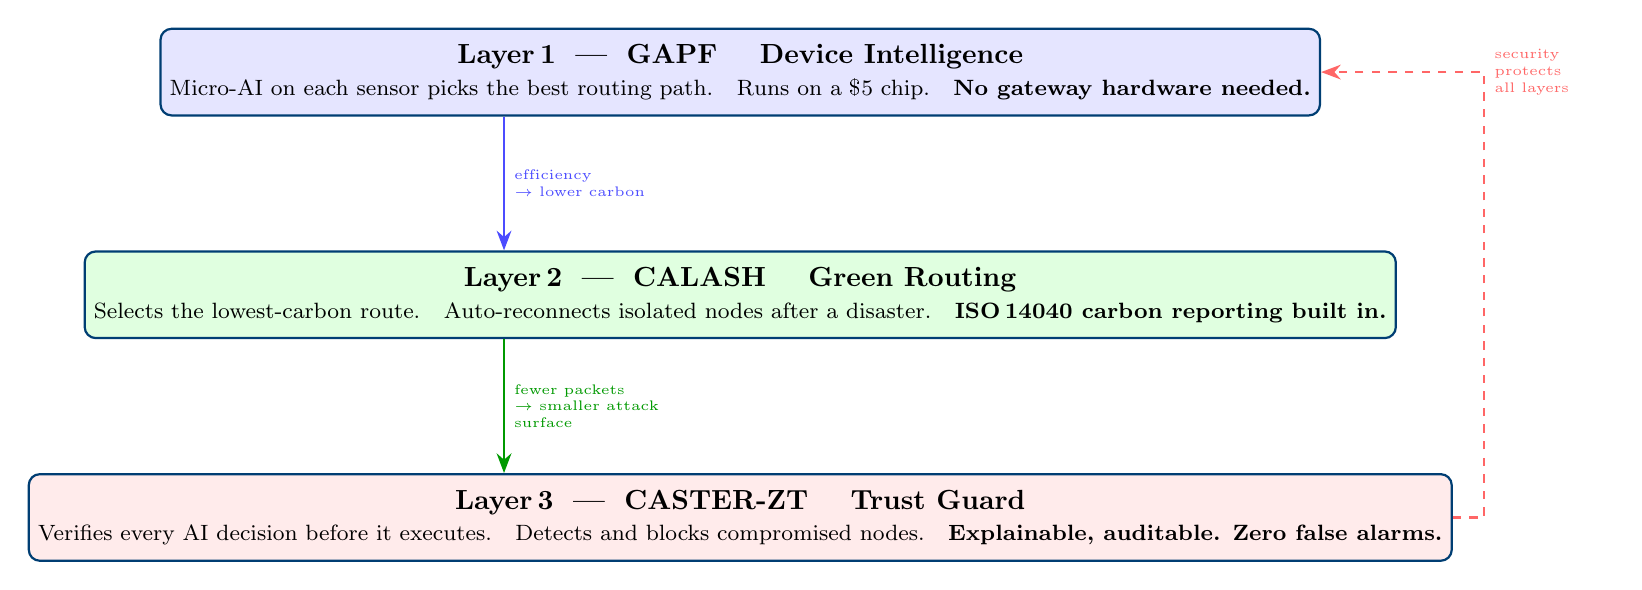
\begin{tikzpicture}[
  box/.style={draw=polyblue, thick, rounded corners=4pt,
              minimum width=9.5cm, minimum height=1.1cm,
              align=center, font=\footnotesize},
  node distance=0pt]

  \node[box, fill=blue!10] (l1) {%
    \textbf{\normalsize Layer\,1 \;---\; GAPF \quad Device Intelligence}\\[2pt]
    Micro-AI on each sensor picks the best routing path.\quad
    Runs on a \$5 chip.\quad \textbf{No gateway hardware needed.}};

  \node[box, fill=green!12, below=1.7cm of l1] (l2) {%
    \textbf{\normalsize Layer\,2 \;---\; CALASH \quad Green Routing}\\[2pt]
    Selects the lowest-carbon route.\quad
    Auto-reconnects isolated nodes after a disaster.\quad
    \textbf{ISO\,14040 carbon reporting built in.}};

  \node[box, fill=red!8, below=1.7cm of l2] (l3) {%
    \textbf{\normalsize Layer\,3 \;---\; CASTER-ZT \quad Trust Guard}\\[2pt]
    Verifies every AI decision before it executes.\quad
    Detects and blocks compromised nodes.\quad
    \textbf{Explainable, auditable. Zero false alarms.}};

  % Down-arrows (left side, well inside box width)
  \draw[-{Stealth[length=2.5mm]}, thick, blue!70]
    ([xshift=-3.0cm]l1.south) -- ([xshift=-3.0cm]l2.north)
    node[midway, right, font=\tiny, text width=2.2cm, align=left]
      {efficiency\\$\to$ lower carbon};
  \draw[-{Stealth[length=2.5mm]}, thick, green!60!black]
    ([xshift=-3.0cm]l2.south) -- ([xshift=-3.0cm]l3.north)
    node[midway, right, font=\tiny, text width=2.2cm, align=left]
      {fewer packets\\$\to$ smaller attack surface};

  % Feedback arrow (right side) — total right extent = 4.75+0.4 = 5.15 cm from
  % slide centre; label adds 1.4 cm more = 6.55 cm < 7.4 cm text half-width
  \draw[-{Stealth[length=2.5mm]}, thick, dashed, red!60]
    (l3.east) -- ++(0.4,0) |- (l1.east)
    node[pos=0.5, right, font=\tiny, text width=1.4cm, align=left]
      {security\\protects\\all layers};
\end{tikzpicture}
\vspace{4pt}
\begin{exampleblock}{}
  \centering\small
  The three layers \textbf{reinforce each other}. Deployed together on one microcontroller,
  they cover network lifetime, carbon sustainability, and AI safety ---
  with \textbf{no trade-off} between the three objectives.
\end{exampleblock}
\end{frame}

% ----------------------------------------------------------
\begin{frame}[shrink=5]{Validation Methodology}
\begin{columns}[T]
\begin{column}{0.50\textwidth}
  \begin{block}{\faGlobe\; How We Built and Tested}
    \begin{itemize}\small\setlength{\itemsep}{4pt}
      \item Designed three AI tools and stress-tested them
            in thousands of simulated disaster scenarios
            (earthquakes, cascading node failures, cyberattacks)
      \item Each tool independently published in
            \textbf{peer-reviewed IEEE journals}:\\
            GAPF and CALASH in \textit{IEEE TGCN},\\
            CASTER-ZT in \textit{IEEE TMC}
      \item Combined: \textbf{more than 23,800 test runs}
            across three independent studies
    \end{itemize}
  \end{block}
\end{column}
\begin{column}{0.47\textwidth}
  \begin{block}{\faCheck\; Three Real-World Data Sources}
    \begin{itemize}\small\setlength{\itemsep}{4pt}
      \item \textbf{Sensor behaviour:}
            Intel Research Lab real sensor traces
            (temperature, humidity, voltage)
      \item \textbf{Carbon intensity:}
            UK National Grid live carbon API
            (real grid emissions over time)
      \item \textbf{Disaster geometry:}
            USGS ShakeMap from the Turkey-Syria earthquake
            (Mw\,7.8, February 2023)
    \end{itemize}
  \end{block}
  \vspace{3pt}
  \begin{alertblock}{Scope}
    \small Results are simulation-based.
    Hardware validation (Zolertia RE-Mote, Google Coral)
    is the planned next step.
  \end{alertblock}
\end{column}
\end{columns}
\end{frame}

% ============================================================
\section{Results}
% ============================================================

\begin{frame}[shrink=5]{Result 1 --- GAPF: Networks That Survive Disasters}
\begin{columns}[T]
\begin{column}{0.50\textwidth}
  \begin{block}{\faBolt\; What GAPF Delivers}
    \begin{itemize}\small\setlength{\itemsep}{3pt}
      \item Each sensor runs a micro-AI that learns
            the best routing path for its battery level and position
      \item The entire AI fits in \textbf{5.8\,KB} ---
            smaller than a text message
      \item No expensive relay gateway is needed:
            the intelligence lives \emph{on} the sensor
    \end{itemize}
  \end{block}
  \vspace{3pt}
  \begin{exampleblock}{\faBriefcase\; Business Translation}
    \begin{itemize}\small\setlength{\itemsep}{2pt}
      \item \textbf{Fewer truck rolls:} sensors last 2--3.5$\times$ longer
      \item \textbf{Lower CAPEX:} no relay gateways to buy or install
      \item \textbf{Coverage guarantee:} 98\% data delivery
            even under full disaster load
    \end{itemize}
  \end{exampleblock}
\end{column}
\begin{column}{0.47\textwidth}
  \centering\small
  \renewcommand{\arraystretch}{1.35}
  \begin{tabular}{lcc}
    \toprule
    \textbf{Metric} & \textbf{Best prior} & \textbf{GAPF} \\
    \midrule
    Data delivery   & 46--67\%      & \textbf{$\geq$\,98\%} \\
    Energy/packet   & $1.0\times$   & \textbf{0.3--0.5$\times$} \\
    AI model size   & $\sim$39K     & \textbf{1,473 params} \\
    Training memory & 3.2--14\,GB   & \textbf{951\,MB} \\
    \bottomrule
  \end{tabular}
  \vspace{8pt}
  \begin{block}{}
    \centering\small
    \textbf{26$\times$ lighter} AI model\\
    than the best competing approach,\\
    yet \textbf{more reliable} on every metric
  \end{block}
\end{column}
\end{columns}
\end{frame}

% ----------------------------------------------------------
\begin{frame}[shrink=12]{Result 2 --- CALASH: Networks That Stay Green}
\begin{columns}[T]
\begin{column}{0.50\textwidth}
  \begin{block}{\faLeaf\; What CALASH Delivers}
    \begin{itemize}\small\setlength{\itemsep}{2pt}
      \item Introduces the first \textbf{carbon intensity metric}
            for wireless sensor networks ---
            fully \textbf{ISO\,14040 compliant}
      \item Routes data through the path with the
            \textbf{lowest carbon cost}, not just the shortest hop
      \item Uses 6G links to \textbf{reconnect isolated nodes automatically}
            after a disaster, with no human intervention
    \end{itemize}
  \end{block}
  \vspace{1pt}
  \begin{exampleblock}{\faBriefcase\; Business Translation}
    \begin{itemize}\small\setlength{\itemsep}{1pt}
      \item \textbf{ESG reporting:} ready-made KPI for
            CSRD and SEC sustainability requirements
      \item \textbf{60\% longer network lifetime}
            reduces maintenance cycles
      \item \textbf{33\% less CO\textsubscript{2} per packet} ---
            auditable for regulators and investors
    \end{itemize}
  \end{exampleblock}
\end{column}
\begin{column}{0.47\textwidth}
  \centering
  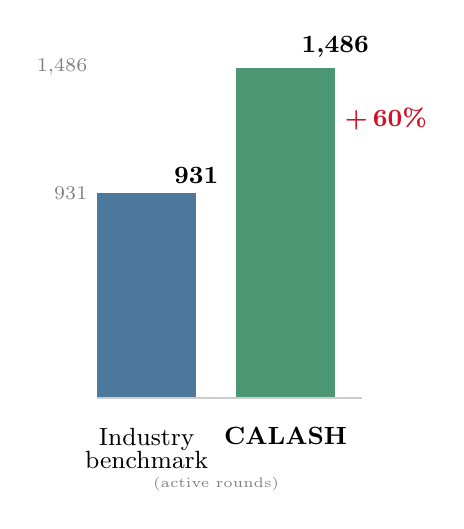
\begin{tikzpicture}[scale=0.84]
    \fill[polyblue!70] (0,0) rectangle (1.5,3.1)
      node[above, font=\small\bfseries, text=black]{931};
    \fill[polygreen!70] (2.1,0) rectangle (3.6,5.0)
      node[above, font=\small\bfseries, text=black]{1,486};
    \node[below, font=\small] at (0.75,-0.3) {Industry};
    \node[below, font=\small] at (0.75,-0.65){benchmark};
    \node[below, font=\small] at (2.85,-0.3) {\textbf{CALASH}};
    \draw[thick, gray!40] (0,0) -- (4.0,0);
    \node[above right, font=\small\bfseries, text=polyred] at (3.6,3.9){+\,60\%};
    \node[left, font=\scriptsize, text=gray] at (0,3.1){931};
    \node[left, font=\scriptsize, text=gray] at (0,5.0){1,486};
    \node[below, font=\tiny, text=gray] at (1.8,-1.05){(active rounds)};
  \end{tikzpicture}
  \vspace{4pt}
  {\centering\scriptsize\color{gray!70}
    Carbon data: \textbf{UK National Grid} real-time API\\[1pt]
    Canadian grid integration: planned pilot step\par}
\end{column}
\end{columns}
\end{frame}

% ----------------------------------------------------------
\begin{frame}[shrink=12]{Result 3 --- CASTER-ZT: Networks That Stay Trustworthy}
\begin{columns}[T]
\begin{column}{0.50\textwidth}
  \begin{block}{\faLock\; What CASTER-ZT Delivers}
    \begin{itemize}\small\setlength{\itemsep}{2pt}
      \item Acts as an \textbf{always-on safety guardrail}:
            every AI decision is verified before it executes
      \item Five graduated responses (monitor $\to$ correct $\to$ defer
            $\to$ escalate $\to$ block) give
            \textbf{proportional, auditable} reactions
      \item The safety layer is \textbf{fully explainable}:
            no black box; every decision is traceable
    \end{itemize}
  \end{block}
  \vspace{1pt}
  \begin{exampleblock}{\faBriefcase\; Business Translation}
    \begin{itemize}\small\setlength{\itemsep}{1pt}
      \item \textbf{0 false alarms:} no service disruption from over-blocking
      \item \textbf{3\,ms per decision:}
            within real-time radio budget (O-RAN limit: 10\,ms)
      \item \textbf{Certification path:} auditable design aligned with
            IEC\,62443 and NIST\,SP\,800-207
    \end{itemize}
  \end{exampleblock}
\end{column}
\begin{column}{0.47\textwidth}
  \centering\small
  \renewcommand{\arraystretch}{1.35}
  \begin{tabular}{lcc}
    \toprule
    \textbf{Metric} & \textbf{Best prior} & \textbf{CASTER-ZT} \\
    \midrule
    Threat detection  & 60--84\%    & \textbf{74--98\%} \\
    False alarms      & 48.8\%      & \textbf{0\%} \\
    Decision latency  & $>$15\,ms   & \textbf{3.07\,ms} \\
    Recovery score    & 0.14--0.20  & \textbf{0.733} \\
    \bottomrule
  \end{tabular}
  \vspace{6pt}
  {\centering\scriptsize\color{gray!70}
    Tested over \textbf{2,420 scenarios} across 100-cell hexagonal networks\\[1pt]
    Recovery \textbf{3.7--5.2$\times$ better} than best competing approach\par}
\end{column}
\end{columns}
\end{frame}

% ============================================================
\section{Business Value and Path Forward}
% ============================================================

\begin{frame}[shrink=8]{Business Value for Mobility Operators}
\centering
\renewcommand{\arraystretch}{1.45}
\begin{tabular}{>{\bfseries\small}p{2.5cm}
                >{\small}p{3.05cm}
                >{\small}p{3.05cm}
                >{\small}p{3.05cm}}
  \toprule
  \textbf{Priority} & \textbf{GAPF} & \textbf{CALASH} & \textbf{CASTER-ZT} \\
  \midrule
  \rowcolor{blue!7}
  Reduce OPEX &
    2--3.5$\times$ longer battery life $\Rightarrow$ fewer field crews &
    +60\% network lifetime $\Rightarrow$ fewer maintenance cycles &
    Near-zero manual interventions per security event \\
  \rowcolor{green!7}
  Reduce CAPEX &
    No relay gateways; runs on \$5 sensor chips &
    Reuses existing 6G and O-RAN infrastructure &
    Runs on same microcontroller as GAPF \\
  \rowcolor{yellow!8}
  ESG \& Sustainability &
    26$\times$ lighter AI $\Rightarrow$ less compute energy &
    ISO\,14040 carbon KPI ready for CSRD / SEC &
    Explainable decisions support ESG governance \\
  \rowcolor{red!5}
  Regulatory \& Safety &
    98\% delivery in disaster zones &
    Standardisable metric (ISO, 3GPP, O-RAN) &
    IEC\,62443 / NIST\,SP\,800-207 path \\
  \bottomrule
\end{tabular}
\vspace{5pt}
\begin{exampleblock}{}
  \centering\small
  All three tools fit together on \textbf{one microcontroller} (103\,KB total).
  They are \textbf{complementary}: efficiency, sustainability, and safety reinforce each other.
  All algorithms are \textbf{open-access with no vendor lock-in}
  (thesis published by Polytechnique Montr\'eal).
\end{exampleblock}
\end{frame}

% ----------------------------------------------------------
\begin{frame}[shrink=5]{Path Forward}
\begin{columns}[T]
\begin{column}{0.31\textwidth}
  \begin{block}{\faCalendar\; 1--2 Years}
    \begin{itemize}\small\setlength{\itemsep}{3pt}
      \item Integrate GAPF, CALASH, and CASTER-ZT
            into a \textbf{unified operational stack}
      \item \textbf{Hardware pilot} on real equipment
            (Zolertia RE-Mote, Google Coral)
            to confirm lab results in the field
      \item Extend disaster models to cascading
            events and wildfires
    \end{itemize}
  \end{block}
\end{column}
\begin{column}{0.31\textwidth}
  \begin{block}{\faCalendar\; 2--4 Years}
    \begin{itemize}\small\setlength{\itemsep}{3pt}
      \item Deploy as \textbf{O-RAN apps} (rApps and xApp)
            on open RAN infrastructure
      \item Distributed AI training across multiple
            operator networks, without sharing raw data
      \item Formal certification of the safety layer
            (IEC\,61508)
    \end{itemize}
  \end{block}
\end{column}
\begin{column}{0.31\textwidth}
  \begin{block}{\faCalendar\; 4+ Years}
    \begin{itemize}\small\setlength{\itemsep}{3pt}
      \item Integrate \textbf{satellite and drone} backhaul
            (LEO, HAPS) for post-disaster coverage
            in any geography
      \item Submit LCI carbon metric and zero-trust
            framework to \textbf{ISO, 3GPP, O-RAN Alliance}
            for standardisation
    \end{itemize}
  \end{block}
\end{column}
\end{columns}
\vspace{5pt}
{\centering\small\textbf{Transfer domains:}
  Precision agriculture \quad Smart cities \quad
  Connected health \quad Vehicle and drone networks\par}
\end{frame}

% ============================================================
%  THANK YOU
% ============================================================
{
\setbeamertemplate{footline}{}
\begin{frame}[plain]
\vfill
\begin{center}
  
\includegraphics[height=1.0cm]{Polytechnique_Montreal_Logo.png}\hspace{2cm}%
  
\includegraphics[height=1.0cm]{Larim_logo.png}

  \vspace{0.5cm}
  {\Huge \textbf{Thank You!}}

  \vspace{0.35cm}
  {\LARGE Questions?}

  \vspace{0.6cm}
  {\large Georges Parfait \textsc{Djimefo Kapen}}\\[4pt]
  {\small Director: \textbf{Ranwa Al-Mallah}}\\[1pt]
  {\small Co-director: \textbf{Samuel Pierre}}\\[1pt]
  {\small Supervisor: \textbf{Franjieh El-Khoury}}\\[5pt]
  {\small Department of Computer and Software Engineering \quad
          Polytechnique Montr\'{e}al~--~LARIM}

  \vspace{0.4cm}
  {\small\color{polyblue}\emph{%
    AI-Driven Intelligent Routing and Secure Autonomous Recovery\\
    in 6G-Integrated Disaster-Monitoring Sensor Networks}}\\[2pt]
  {\footnotesize Friday, May 15, 2026}
\end{center}
\vfill
\end{frame}
}

% ============================================================
%  BACKUP SLIDES
% ============================================================
\appendix
\begin{frame}[plain]
  \centering{\Large \textbf{Backup Slides}}\\[4pt]
  {\small Detailed results --- available on request}
\end{frame}

% ----------------------------------------------------------
\begin{frame}[shrink=15]{Full Quantitative Summary --- All Three Studies}
\centering\small
\renewcommand{\arraystretch}{1.2}
\begin{tabular}{@{}llccc@{}}
  \toprule
  \textbf{Metric} & \textbf{Best prior approach} & \textbf{Prior value}
    & \textbf{Our result} & \textbf{Gain} \\
  \midrule
  Data delivery rate  & QMIX (RL agent) & 46--67\%    & $\geq$\,\textbf{98\%}  & +43--111\% \\
  Energy per packet   & QMIX            & $1.0\times$ & $0.3$--$0.5\times$     & 2--3.5$\times\downarrow$ \\
  AI model parameters & RNN agent       & $\sim$39K   & \textbf{1,473}         & 26$\times\downarrow$ \\
  Training memory     & QMIX            & 3.2--14\,GB & \textbf{951\,MB}       & 3.4--14.5$\times\downarrow$ \\
  Network lifetime    & LEACH           & 931 rounds  & \textbf{1,486 rounds}  & +60\% \\
  Carbon per packet   & LEACH           & 13.42       & \textbf{8.99}          & $-$33\% \\
  Threat detection    & Best 0-FP ref.  & 0\%         & \textbf{74--98\%}      & +74--98\,pts \\
  False alarms        & Shield-Binary   & 48.8\%      & \textbf{0\%}           & Eliminated \\
  Decision latency    & O-RAN budget    & 10\,ms      & \textbf{3.07\,ms}      & 3.3$\times\downarrow$ \\
  Criteria covered    & Best existing   & 1\,/\,12    & \textbf{12\,/\,12}     & 12$\times\uparrow$ \\
  \midrule
  \multicolumn{4}{l}{\textbf{Total test runs across all three studies}}
    & \textbf{$>$23,800} \\
  \bottomrule
\end{tabular}
\vspace{5pt}
\begin{exampleblock}{}
  \centering\small
  The complete AI stack uses \textbf{$\sim$27,000 parameters} and fits in
  \textbf{103\,KB} --- on a microcontroller costing a few dollars.
  This is \textbf{38$\times$ lighter} than MCUNet,
  the current reference for AI on embedded chips.
\end{exampleblock}
\end{frame}

% ----------------------------------------------------------
\begin{frame}{UN Sustainable Development Goals Alignment}
\centering\small
\renewcommand{\arraystretch}{1.3}
\begin{tabular}{cll}
  \toprule
  \textbf{SDG} & \textbf{Target} & \textbf{Contribution} \\
  \midrule
  \textbf{9}  & Resilient infrastructure, innovation       & Ultra-light routing AI (1,473 params) \\
  \textbf{11} & Reduce disaster losses (target 11.5)       & 98\% data delivery + automatic self-healing \\
  \textbf{12} & Sustainability reporting (target 12.6)     & ISO\,14040 carbon KPI for IoT networks \\
  \textbf{13} & Climate resilience (target 13.1)           & Carbon-aware routing + post-disaster recovery \\
  \textbf{16} & Transparent institutions (target 16.6)     & Explainable safety shield + 0 false alarms \\
  \bottomrule
\end{tabular}
\vspace{8pt}
\begin{columns}[T]
\begin{column}{0.48\textwidth}
  \begin{block}{Sendai Framework for Disaster Risk Reduction}
    \small Directly addresses \textbf{indicators C-2}
    (communication and warning systems) and \textbf{C-6}
    (early warning infrastructure) of the UN Sendai Framework 2015--2030.
  \end{block}
\end{column}
\begin{column}{0.48\textwidth}
  \begin{block}{Standardisation Pathway}
    \small LCI metric is a candidate for \textbf{ISO TC\,207/SC\,7}.
    GAPF and CALASH are proposed as rApps for
    \textbf{O-RAN Alliance WG2}.
    CASTER-ZT maps to \textbf{3GPP SA5} AI/ML trust requirements.
  \end{block}
\end{column}
\end{columns}
\end{frame}

\end{document}
